\documentclass[12pt,a4paper]{report}

\usepackage[backend=biber, style=ieee]{biblatex}
\addbibresource{literature.bib}

\usepackage[utf8]{inputenc}
\usepackage[T1]{fontenc}
\usepackage[ngerman]{babel}
\usepackage{lmodern}
\usepackage{enumitem}
\usepackage{graphicx}
\usepackage{tabularx}
\usepackage{float}
\usepackage[onehalfspacing]{setspace}
\usepackage{microtype}
\usepackage{parskip}
\usepackage{minted}

\usepackage{xcolor}
\newcommand{\todo}[1]{\colorbox{red}{\textbf{TODO: #1}}\\}
\newcommand{\question}[1]{\colorbox{yellow}{\textbf{QUESTION: #1}}\\}
\newcommand{\xeno}[1]{\colorbox{pink}{\textbf{TODO XENO: #1}}\\}
\newcommand{\gideon}[1]{\colorbox{green}{\textbf{TODO GIDEON: #1}}\\}

\begin{document}

\tableofcontents
\newpage

\section{IntelliJ IDEA Companion}

Die Implementierung nutzt die von JetBrains bereitgestellten IntelliJ-Plugin-APIs, um sich direkt in den Entwicklungsablauf der
IDE einzuklinken. Diese APIs ermöglichen es, Ereignisse wie einen erfolgreichen Code-Commit abzufangen, eigene Dialogfenster oder
Benachrichtigungen anzuzeigen und auf gespeicherte Plugin-Einstellungen zuzugreifen. Dadurch kann das Yappi Companion-Plugin
nahtlos in die bestehende IntelliJ-Oberfläche integriert werden, ohne den gewohnten Workflow der Entwickler zu unterbrechen.

Der IntelliJ Companion erweitert Yappi um die Möglichkeit, direkt aus der Entwicklungsumgebung heraus Feedback zu Code-Commits
zu erfassen. Ziel ist es, die Erfassung von Stimmungsdaten möglichst nahtlos in den Entwickler-Workflow zu integrieren, ohne den
Arbeitsfluss zu unterbrechen. Nach jedem erfolgreichen Commit in IntelliJ IDEA öffnet sich automatisch ein Dialogfenster, in dem
der Entwickler seine Stimmung zum Commit angeben kann. Diese Daten werden anschliessend an Yappi übertragen und dort gespeichert.

\subsection{Architektur und Integration}

Dia Abbildung~\ref{fig:intellij-system-diagram} zeigt den Aufbau des Yappi IntellJ IDEA Companion.

\begin{figure}[H]
\centering
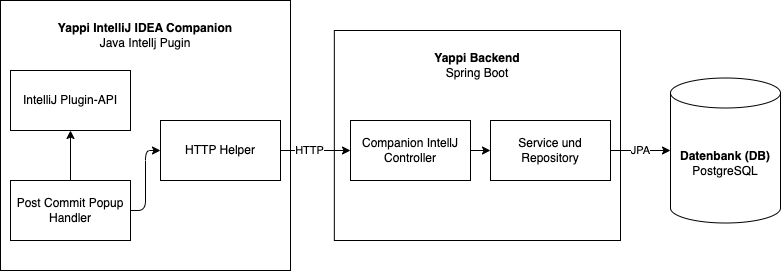
\includegraphics[width=0.95\textwidth]{../figures/intellij-system-diagram.drawio.png}
\caption{Architektur des IntelliJ IDEA Companion}
\label{fig:intellij-system-diagram}
\end{figure}

Die Implementierung basiert auf den IntelliJ-Plugin-APIs. Ein (\texttt{PostCommitPopupHandler}) registriert sich auf erfolgreiche
Commit-Events. Nach Bestätigung des Commits wird der Post-Commit Dialog angezeigt. Der API-Key, der zur Authentifizierung
gegenüber Yappi benötigt wird, wird über die Plugin-Einstellungen eingegeben und in einer persistenten Komponente
(\texttt{CompanionStorage}) gespeichert. Die Kommunikation mit dem Backend erfolgt über eine dedizierte Hilfsklasse
(\texttt{HttpHelper}), welche die Daten an den entsprechenden Endpoint überträgt.

\subsection{Speicherung der Einstellungen}

Damit sich die Companion App Authentifizieren kann muss ein gültiger API Key hinterlegt werden. Die Eingabe des API-Keys erfolgt
über den Menüpunkt Settings → Tools → Yappi Companion in IntelliJ. Die Abbildung~\ref{fig:intellij-settings} zeigt den 
entsprechenden Menupunkt.

\begin{figure}[H]
\centering
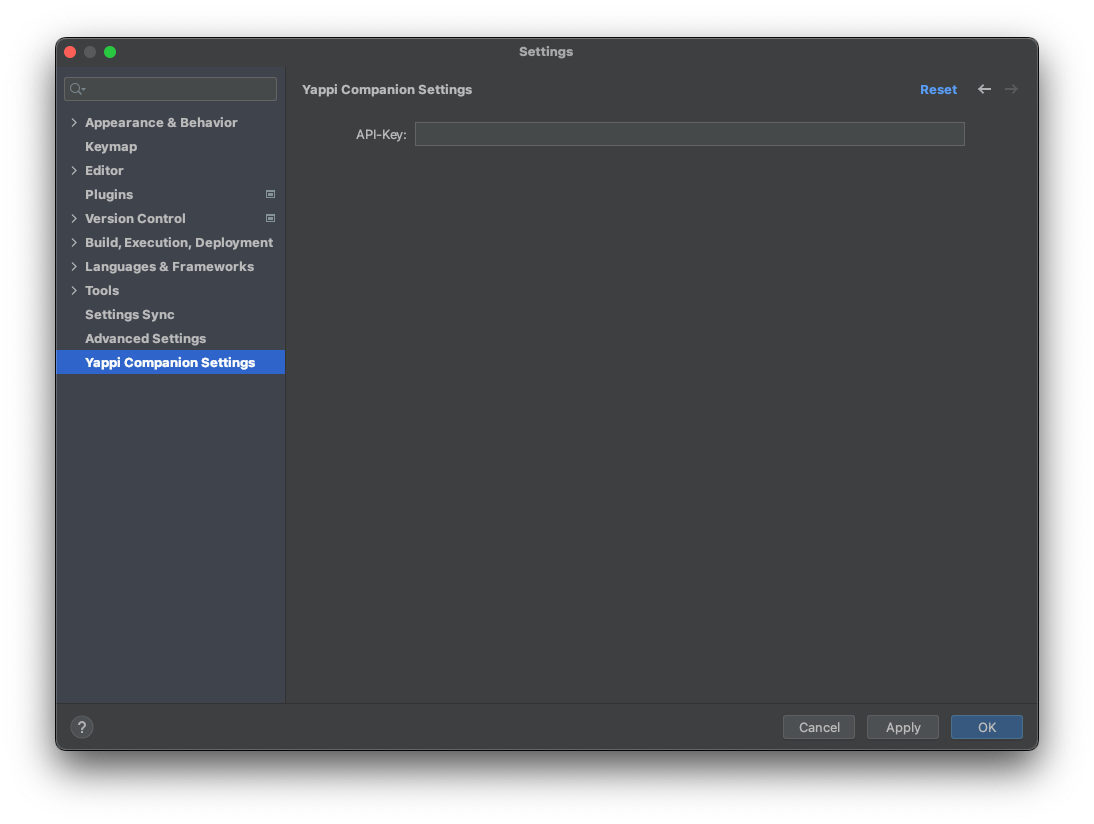
\includegraphics[width=0.95\textwidth]{../figures/intellij-settings.png}
\caption{Eingabe des API-Keys in den IntelliJ Companion-Einstellungen}
\label{fig:intellij-settings}
\end{figure}

Der Key wird in der Klasse \texttt{CompanionStorage} mithilfe der IntelliJ-Persistenzmechanismen gespeichert und beim nächsten
Start automatisch geladen.

\subsection{Post-Commit Dialog}

Das Post-Commit-Popup wird automatisch unmittelbar nach einem erfolgreichen Commit in IntelliJ IDEA angezeigt. Ziel ist es, die
Erfassung von Stimmungsdaten so nahtlos wie möglich in den normalen Entwicklungs- und Versionskontrollprozess einzubinden. Der
Dialog öffnet sich als eigenständiges Fenster und blockiert die IDE nicht, sodass Entwickler sofort weiterarbeiten können. Die
Abbildung~/ref{fig:intellij-post-commit} zeigt die Benutzeroberfläche.

\todo{neues design}
\begin{figure}[H]
\centering
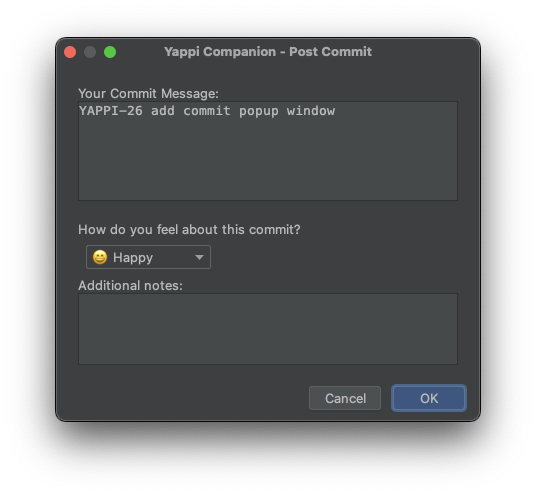
\includegraphics[width=0.95\textwidth]{../figures/intellij-post-commit.png}
\caption{Post-Commit Dialog des IntelliJ Companions}
\label{fig:intellij-post-commit}
\end{figure}

Die Benutzeroberfläche umfasst zwei zentrale Elemente:

\begin{itemize}
  \item \textbf{Commit-Nachricht:} Im oberen Bereich wird die soeben erfasste Commit-Nachricht angezeigt.
  \item \textbf{Stimmungsauswahl:} Über ein Dropdown-Menü können vordefinierte Stimmungen ausgewählt werden, jeweils ergänzt durch
    ein Emoji zur schnellen Orientierung.
\end{itemize}

Nach Bestätigung des Dialogs werden die eingegebenen Daten an das Yappi-Backend gesendet. Dieser Vorgang läuft vollständig im
Hintergrund ab, sodass der Entwickler direkt mit seiner Arbeit fortfahren kann.

\subsection{Daten verarbeiten und Persistieren}

Die vom IntelliJ Companion erfassten Commit-Daten werden über eine gesicherte Verbindung an das Yappi-Backend übertragen. Dort
erfolgt zunächst die Authentifizierung anhand des API-Keys, der zuvor in den Plugin-Einstellungen hinterlegt wurde. Anschliessend
werden die empfangenen Daten verarbeitet und persistiert.

\subsubsection{Backend-Komponente}

Für die Verarbeitung wurde eine eigene Backend-Komponente entwickelt, bestehend aus einem neuen Controller, einem Service und
einem Repository für den Datenbankzugriff. 

Der Controller \texttt{IntellijCompanionController} stellt den Endpoint, über den die Zufriedenzeitsdaten und commit-spezifischen
Kontextinformationen entgegengenommen werden, bereit. Der Endpoint ist volgendermassen aufgebaut.

\begin{description}
  \item \texttt{POST /companion/commit} \\
        Erfasst Zufriedenheitsdaten inklusive Kontexinformationen nach einem Commit. \\
        \textbf{Antworten:} \texttt{200 OK}, \texttt{400 Bad Request}, \texttt{401 Unauthorized}.
\end{description}

Die Speicherung erfolgt über ein Repository, das direkt auf die Datenbank zugreift.

\subsubsection{Datenbankerweiterung}

Die vom IntelliJ Companion übermittelten Zufriedenheitsdaten werden im Backend zusammen mit den zusätzlichen Kontextinformationen
persistiert. Während die eigentlichen Stimmungsdaten in der bestehenden Tabelle für Zufriedenheitsmessungen gespeichert werden,
wird für die Commit-bezogenen Zusatzinformationen eine separate, flexible Kontexttabelle angelegt. Diese Trennung erlaubt es, in
Zukunft weitere Arten von Kontextdaten ohne Änderungen Datenbankschama der Zufriedenheitsdaten zu integrieren.

Die Tabelle~\ref{tab:commit_context_schema} zeigt den Aufbau der neuen Kontexttabelle \texttt{commit\_context}.

\begin{table}[H]
\centering
\begin{tabular}{|l|l|p{9cm}|}
\hline
\textbf{Spalte} & \textbf{Datentyp} & \textbf{Beschreibung} \\
\hline
\texttt{id} & SERIAL & Primärschlüssel, auto-inkrementierend \\ 
\texttt{satisfaction\_id} & INTEGER & Fremdschlüssel auf \texttt{satisfaction\_data.id}, verknüpft die Kontextdaten mit einer 
  Zufriedenheitsmessung \\
\texttt{context\_type} & TEXT & Die Art von Kontextinformation die gespeichert wird (z.B. Commit-Message oder Number of Lines 
  Changed) \\
\texttt{value} & TEXT & Der Wert welcher gespeichert wird. Z.B. die Commit-Nachricht, wie sie in IntelliJ beim Commit eingegeben
  wurde \\
\texttt{created\_at} & TIMESTAMPTZ & Zeitpunkt, zu dem der Datensatz erstellt wurde \\
\hline
\end{tabular}
\caption{Schema der Tabelle \texttt{commit\_context}}
\label{tab:commit_context_schema}
\end{table}

Die Speicherung in einer separaten Tabelle stellt sicher, dass die Kernlogik der Zufriedenheitsmessungen unverändert bleibt,
während gleichzeitig ein flexibles Datenmodell für kontextbezogene Informationen zur Verfügung steht. Dadurch lässt sich der
Funktionsumfang von Yappi künftig unkompliziert erweitern, ohne bestehende Datenstrukturen zu beeinträchtigen.

\printbibliography

\end{document}
